\begin{frame}{LIME on Text: Finding a Shortcut}

    \centering
    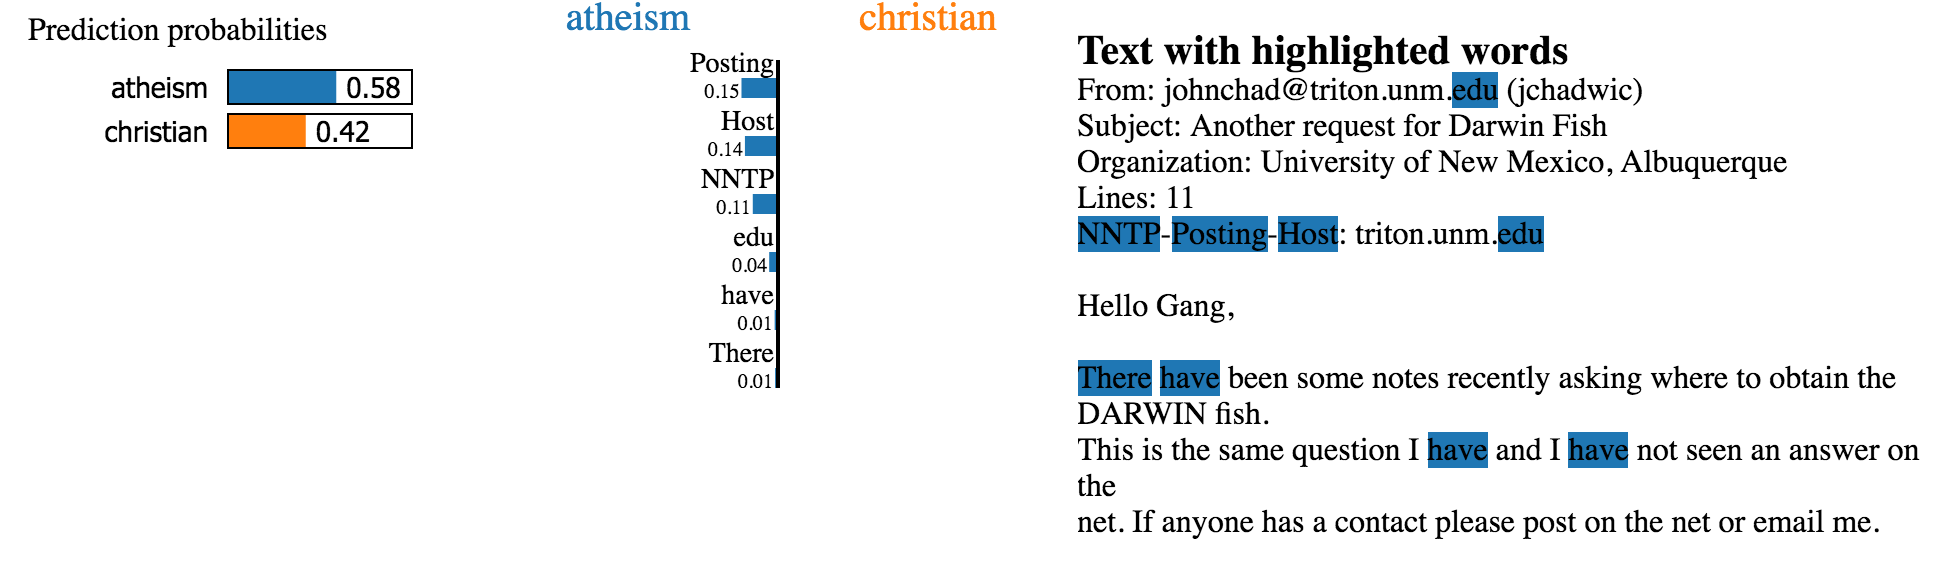
\includegraphics[width=0.83\textwidth,height=0.40\textheight,keepaspectratio]{images/responsible-ai/lime_text_twoclass_explanation.png}

    \vspace{0.3em}
    {\scriptsize Source: \texttt{lime} library documentation,
    \href{https://github.com/marcotcr/lime}{github.com/marcotcr/lime}
    (\texttt{doc/images/twoclass.png}); 20 Newsgroups atheism-vs-christianity classifier.}

    \vspace{0.5em}
    \raggedright
    \begin{itemize}\small
        \setlength\itemsep{0.3em}
        \item The classifier reports 0.58 for ``atheism.'' The explanation shows the evidence:
              \texttt{Posting}, \texttt{Host}, \texttt{NNTP}, \texttt{edu} --- \textbf{email header
              artefacts}, not content.
        \item This is the single most valuable use of local explanations: a high-accuracy model
              that is right for a reason that will not survive contact with new data.
        \item You would never have found it from the accuracy score.
    \end{itemize}
\end{frame}

\begin{frame}{LIME on Images}

    \centering
    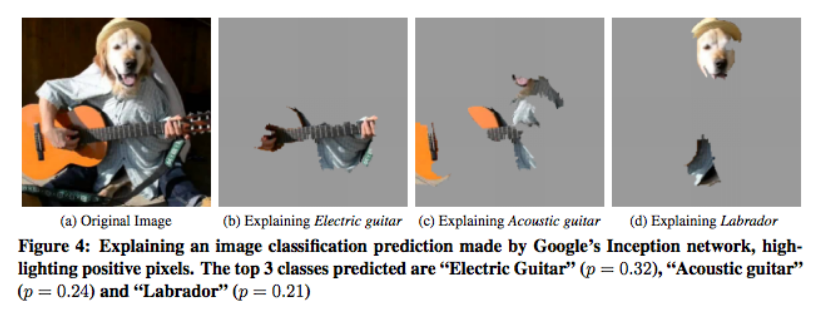
\includegraphics[width=0.78\textwidth,height=0.40\textheight,keepaspectratio]{images/responsible-ai/lime_paper_fig4_image_explanations.png}

    \vspace{0.3em}
    {\scriptsize Source: Figure 4 of M.~T.~Ribeiro, S.~Singh and C.~Guestrin, ``\,`Why Should I
    Trust You?': Explaining the Predictions of Any Classifier,'' KDD 2016
    (\href{https://arxiv.org/abs/1602.04938v3}{arXiv:1602.04938v3}), as reproduced in the
    \href{https://github.com/marcotcr/lime}{\texttt{lime}} repository.}

    \vspace{0.6em}
    \raggedright
    \begin{itemize}\small
        \setlength\itemsep{0.3em}
        \item The image is segmented into superpixels; perturbation switches groups of them off.
        \item Each panel shows the superpixels supporting a \emph{different} predicted class ---
              the explanation is always \textbf{relative to a target class}, never absolute.
        \item Useful check: if the supporting region is the background rather than the object, you
              have found a dataset artefact.
    \end{itemize}
\end{frame}
